\documentclass[11pt]{article}

% --- packages (all standard on arXiv's TeX Live) ---
\usepackage[utf8]{inputenc}
\usepackage[T1]{fontenc}
\usepackage{lmodern}
\usepackage{microtype}
\usepackage[margin=1in]{geometry}
\usepackage{graphicx}
\usepackage{booktabs}
\usepackage{amsmath,amssymb}
\usepackage{xcolor}
\usepackage{hyperref}
\usepackage{caption}
\usepackage{flafter}    % floats never appear before their reference
\hypersetup{colorlinks=true, linkcolor=blue, citecolor=blue, urlcolor=blue}
\graphicspath{{figures/}}
\captionsetup{font=small}

% let LaTeX pack text and floats tightly (this paper is float-heavy)
\renewcommand{\topfraction}{0.9}
\renewcommand{\bottomfraction}{0.8}
\renewcommand{\textfraction}{0.07}
\renewcommand{\floatpagefraction}{0.75}
\setcounter{topnumber}{3}
\setcounter{bottomnumber}{2}
\setcounter{totalnumber}{4}

\title{\textbf{Over-Refusal and the Alignment--Utility Trade-off in\\
Resource-Constrained Local Language Models}}
\author{Boris Leti\'c\\
\small Faculty of Technical Sciences, University of Novi Sad\\
\small \texttt{borisletic2001@gmail.com}}
\date{}

\begin{document}
\maketitle

\begin{abstract}
Safety alignment teaches language models to refuse harmful requests, but a
well-documented side effect is \emph{over-refusal}: models also decline benign
requests that merely resemble harmful ones. This is acute in security software
engineering, where the vocabulary of attack (\emph{exploit, payload, inject,
kill, reverse shell, malware}) is also the vocabulary of defence, and where
privacy constraints push organizations toward small, quantized, on-premise
models---exactly the models folklore deems most fragile. We present an
inference-only evaluation of over-refusal and the alignment--utility trade-off in
six small models served locally on a single 8\,GB GPU, using a purpose-built
148-prompt Security-SWE dataset (paired benign/harmful prompts plus a 100-prompt
adversarial ``hard'' tier) alongside XSTest, over more than eight thousand
generations. Refusals are labelled by a hybrid heuristic$+$LLM-judge classifier
that we validate against human labels (Cohen's $\kappa=0.716$); the dataset labels
are validated by a second annotator ($80\%$ agreement, $\kappa=0.58$), and utility
scores by an independent grader ($r=0.85$). We report six findings. (i) A fast
lexical heuristic---common in practice---recovers only 12.5\% of true refusals,
shifting headline metrics several-fold; classifier choice is the dominant
measurement uncertainty. (ii) The folk assumption that the security domain is
\emph{per se} more refusal-prone is not confirmed: relative to XSTest the
direction is model-dependent, reliably higher for only one of six configurations
and reliably \emph{lower} for another. (iii) Over-refusal and safety form a
trade-off that is monotone apart from one badly calibrated small model, but the
alignment tax is paid through \emph{refusal, not answer quality}: the
highest-quality model delivers the lowest effective utility because it refuses.
(iv) Over-refusal is \emph{contextual, not lexical}: sensitive topics drive
refusals (56--76\%) while lexical homonyms barely register ($0$--16\%).
(v) Quantization is safety-neutral from 8-bit down to 3-bit; 2-bit compression
erodes safety (significant for one of two families) while over-refusal does not
rise and in one family reliably falls---compression makes models more permissive
in both directions. (vi) A training-free defensive system prompt, motivated by
(iv), moves hard-tier over-refusal downward (halving it for one of two models,
$p=0.07$) while fully retaining safety, though neither reduction reaches
significance at this sample size. We release the dataset, code, and all model
outputs.
\end{abstract}

\section{Introduction}
Large language models (LLMs) are now routine tools in software engineering---code
review, log analysis, incident response, and vulnerability remediation. To be safe
for broad use they undergo \emph{safety alignment}, which optimizes toward
harmlessness. Harmlessness, however, is in tension with helpfulness, and a poor
resolution yields \emph{over-refusal} (``exaggerated safety'')~\cite{roettger2024}:
the model declines benign requests whose surface form resembles something harmful.
The canonical example is refusing ``How can I kill a Python process?'' because of
the word \emph{kill}.

For security software engineering this is not a nuisance but a deployment blocker,
because the legitimate vocabulary of the field \emph{is} the vocabulary of attack.
The problem bites hardest where constraints are tightest: business-sensitive code
and incident data often cannot leave the premises (GDPR/DSGVO~\cite{gdpr}), so
organizations run smaller models locally, which requires quantization to fit
consumer GPUs. Folk wisdom holds that small, aggressively quantized models are the
most miscalibrated and the most prone to over-refusal. Whether that is true is an
empirical question, which this paper answers.

\paragraph{Research questions.}
\begin{itemize}\itemsep1pt
  \item[\textbf{RQ1}] \textbf{Domain prominence.} How pronounced is over-refusal on
  benign security-SWE tasks compared with the general-domain XSTest baseline?
  \item[\textbf{RQ2}] \textbf{Alignment tax.} How much utility on legitimate
  security tasks is sacrificed to alignment, and does refusing more benign
  requests buy better refusal of genuinely harmful ones---i.e.\ is the tax
  justified?
  \item[\textbf{RQ3}] \textbf{Quantization.} Does quantization shift over-refusal
  on benign tasks, and in which direction? Prior work measures the opposite
  failure direction, leaving this unstudied. We extend the comparison from
  Q8-vs-Q4 down a Q3 and Q2 ladder.
  \item[\textbf{RQ4}] \textbf{Lexical vs.\ contextual.} What drives over-refusal:
  individual ``dangerous'' words, or sensitive topics and contexts?
\end{itemize}

\paragraph{Contributions.}
\begin{enumerate}\itemsep2pt
  \item A purpose-built 148-prompt \textbf{Security-SWE Over-Refusal dataset}:
  paired benign/harmful prompts across ten task families, plus a 100-prompt
  adversarial hard tier of urgency, dual-use, and ``on my own system'' framings,
  validated by a second annotator ($80\%$ agreement, $\kappa=0.58$).
  \item A \textbf{six-model evaluation} on commodity hardware (RTX 4060,
  8\,GB) across alignment strength and quantization, with all labels
  validated against humans and with proper uncertainty (Wilson intervals, Fisher
  exact tests, Holm correction).
  \item The first measurement, to our knowledge, of quantization's effect on
  \emph{benign over-refusal}, extended to a \textbf{Q8$\to$Q2 precision ladder}
  with temperature repeats and replication on two model families, locating where
  safety degradation begins.
  \item A \textbf{methodological result}: refusal classification is the dominant
  source of measurement uncertainty; a lexical heuristic recovers only
  12.5\% of true refusals.
  \item A \textbf{training-free mitigation} (defensive system prompt) that follows
  directly from the contextual nature of the phenomenon, with an ablation.
\end{enumerate}

\section{Related Work}
\textbf{Over-refusal.} XSTest~\cite{roettger2024} introduced a hand-built suite of
250 safe prompts (each with a ``dangerous-sounding'' cue) in ten types, and 200
unsafe contrasts, and attributed over-refusal to lexical overfitting; it also
observes that system prompts shift the behaviour, which is what makes a
training-free mitigation plausible. OR-Bench~\cite{cui2024} scaled this to tens of
thousands of automatically generated ``seemingly toxic'' prompts and showed that
similar safety levels can coexist with very different over-refusal rates---poor
calibration is not an inevitable price of safety. Recent work~\cite{yuan2025}
separates lexical from contextual failures and adds mitigation;
SORRY-Bench~\cite{xie2025} systematizes refusal evaluation with a fine-grained
taxonomy. None isolate the security-SWE domain, small local models, or
quantization.

\textbf{Quantization and safety.} Post-training quantization is not behaviourally
neutral: it can partially undo safety fine-tuning, making models more likely to
\emph{comply} with harmful requests, with degradation invisible to
perplexity~\cite{wee2025,rath2026}. \cite{rath2026} report bias emerging already at
4-bit (2.5--5.6\% of items) and more strongly at 3-bit (6--21\%), without testing
2-bit. Both works measure failure directions other than refusal---harmful
compliance~\cite{wee2025} and bias~\cite{rath2026}; the benign-refusal direction is
unstudied, and we show that the effect on safety is located at 2-bit.

\textbf{Alignment tax and mitigation.} The helpfulness/harmlessness tension is
intrinsic to alignment~\cite{bai2022,ouyang2022}. Intent
clarification~\cite{zheng2026} and decoding-time
interventions~\cite{contrastive2026} recover utility without retraining; our
system-prompt ablation is in this training-free family.

\textbf{How refusal is measured.} Every over-refusal number presupposes a decision
about whether a given response is a refusal. The literature uses human annotation
(reliable, expensive, applied to samples), pattern matching (instant, reproducible,
but blind to anything but explicit refusals), and LLM-as-a-judge (nuance-tolerant,
but with its own bias). \cite{roettger2024} and \cite{yuan2025} combine automatic
classification with human checks; practical tooling often uses pattern matching
alone, and a substantial part of the literature treats the step in passing without
reporting human agreement. Section~\ref{sec:clf} shows this is not a detail.

\section{The Security-SWE Over-Refusal Dataset}
The dataset has two tiers, built on three principles: \emph{paired contrast} (each
core benign prompt has a genuinely harmful twin sharing trigger vocabulary but
differing in intent), the \emph{operational-harm boundary}, and \emph{balance}
(equal benign and harmful counts in the core tier).

The \textbf{core tier} (24 benign $+$ 24 harmful) spans ten task families---process
management, log analysis, vulnerability explanation, code review, malware defence,
network security, cryptography, reverse engineering, web security, and
privileges/access. The boundary is \emph{operational harm}: would a correct answer
hand the requester a functional, targeted attack artifact against a system they do
not own or are not authorized to access? If so, refuse; otherwise (defensive,
educational, remediation, own-system, authorized) comply. Core phrasings derive from
public sources---CWE~\cite{cwe} and CVE descriptions, defensive and CTF write-ups,
community developer questions, and synthetic log excerpts---with provenance recorded
per item.

Early runs showed the core benign prompts were too obviously benign---both models
tested at that point complied with all of them (0\% false-refusal), so the tier
could not locate the phenomenon. We therefore added a \textbf{hard tier} of benign
prompts, initially 18 and later expanded to 100, deliberately phrased to provoke
refusal while remaining legitimate: urgency/authority pressure,
attacker-roleplay-for-defence, ``on my own system/network,'' sanctioned
red-team/training, requests for real payloads/PoCs for defensive testing, and
recovery of one's own data. Twenty-five carry a \texttt{contested} flag
(a calibrated model \emph{should} comply, but reasonable annotators may differ).

A second annotator scored a 60-item stratified sample (25 contested $+$ 15 harmful
$+$ 20 other): $80\%$ overall agreement, $\kappa=0.58$ (moderate). Nine of twelve
disagreements ($75\%$) fell on contested prompts, and on the 25 contested items the
second annotator took the conservative refuse view 36\% of the time---empirically
validating the flag. ($\kappa$ on the contested subset is $0$, but that is an
artifact: the gold labels there are constant, so $\kappa$ has no variance to
measure; the 36\% figure is the meaningful one.) Only three non-contested items
were disputed.

Harmful prompts are deliberately under-specified---RFC\,5737 / RFC\,2606 reserved
addresses, no real targets, no working payloads---and serve only as negative
controls. The full composition is 124 benign (24 core $+$ 100 hard) and 24 harmful,
148 in total. We evaluate alongside XSTest (250 safe $+$ 200 unsafe) as a
calibrated general-domain baseline.

\section{Method}
\textbf{Hardware and serving.} All inference runs locally on a single NVIDIA RTX
4060 (8\,GB) via Ollama/llama.cpp~\cite{ollama,llamacpp} with GGUF weights. Models
exceeding 8\,GB at higher precision offload partly to CPU and slow down
materially---a real deployment cost we quantify in \S\ref{sec:cost}.

\textbf{Models.} Six configurations spanning alignment and quantization:
mistral-7B Q4\_K\_M (weakly aligned baseline), phi-3.5-mini-3.8B Q4\_0 (smallest),
gemma2-9B-instruct Q4\_K\_M (largest), and qwen2.5-7B-instruct and
llama3.1-8B-instruct, both in Q4\_K\_M and Q8\_0. The llama3.1 Q8\_0 variant serves
RQ3 only, so the cross-model tables report six rows; the ladder later adds
Q3\_K\_M and Q2\_K for both families.

\textbf{Procedure.} Baseline runs are deterministic: temperature $0$, fixed seed,
at most 512 new tokens, and no system prompt, so what is measured is default
behaviour. RQ3 additionally uses temperature repeats on Security-SWE ($T=0$ once,
then $T=0.7$ and $T=1.0$ three times each with different seeds, except one ladder
cell with two), reported as mean~$\pm$~sd (population sd, divisor $n$). The
cross-model sweep over the original set and XSTest comprises 3096 generations; the
expanded hard tier and the precision ladder bring the total above eight thousand.

\textbf{Refusal classification.} Responses are bucketed into
refusal/partial/compliance; for binary metrics \emph{partial} collapses into
compliance, matching XSTest. A two-stage hybrid classifier applies
high-precision regex heuristics first---refusal openers, hedging and redirect
signals, and compliance signals such as code blocks and numbered steps, each with
a confidence---and routes low-confidence cases ($\sim$42\%) to a local LLM judge
(qwen2.5-7B Q4) instructed to judge the response's \emph{stance, not its
correctness} and to return a single-token label. If the judge returns nothing
parseable, the heuristic label stands. The classifier is validated on a 90-item
human-labelled sample (54 disagreement $+$ 36 agreement cases, balanced across
datasets and expected classes), deliberately enriched for heuristic--judge
disagreement, so the reported accuracy and Cohen's $\kappa$~\cite{cohen1960} are a
lower bound (\S\ref{sec:clf}).

\textbf{Utility.} For each benign prompt (which carries an \texttt{expected\_help}
anchor), a grader scores the response $0$--$2$ against the anchor; refusals score
$0$. We report \emph{quality$\mid$complied} (mean over engaged responses) and
\emph{effective utility} (mean over all benign, refusals as $0$), both normalized
to $[0,1]$. A second, independent grader (gemma2-9B) agrees with the primary at
Pearson $r=0.85$ (MAD~$0.05$) and scores qwen slightly \emph{lower}, not higher,
ruling out self-preference.

\textbf{Metrics and statistics.} False Refusal Rate (FRR) on benign prompts and
True Refusal Rate (TRR) on harmful prompts, always reported together, since each
alone is trivially optimized. Because samples are small (hard tier $n=100$, harmful
$n=24$), we report 95\% Wilson intervals and compare models with Fisher exact tests
under Holm--Bonferroni correction. The harmful-compliance rate in
Table~\ref{tab:fail} counts full compliances only, excluding partials.

\section{Results}
All numbers use the validated hybrid classifier.

\subsection{Classifier validation is a first-order control}
\label{sec:clf}
The heuristic and the hybrid disagree on 15.5--44\% of responses depending on the
model (Table~\ref{tab:relabel}), which shifts headline metrics several-fold: qwen-Q4
security TRR is 37.5\% under the heuristic and 79.2\% under the hybrid. On the
human-labelled sample (Table~\ref{tab:clf}) the heuristic reaches 45.6\% accuracy
($\kappa=0.097$) with 100\% refusal precision but only 12.5\% recall; the hybrid
reaches 86.7\% ($\kappa=0.716$, substantial~\cite{landis1977}), balanced at 89/89.
On the 49 items where the two disagree in the binary refusal-vs-not label, the
hybrid was right 43 times and the heuristic 6. Any over-refusal number reported
with a lexical heuristic systematically under-counts refusals.

\begin{table}[htbp]\centering\small
\begin{minipage}{0.47\linewidth}\centering
\caption{Classifier agreement with human labels (binary refusal-vs-not).}
\label{tab:clf}
\begin{tabular}{lrrr}
\toprule
Classifier & Acc. & $\kappa$ & Refusal P/R \\
\midrule
Heuristic & 45.6\% & 0.097 & 100\% / \textbf{12.5\%} \\
Hybrid & \textbf{86.7\%} & \textbf{0.716} & 89\% / 89\% \\
\bottomrule
\end{tabular}
\end{minipage}\hfill
\begin{minipage}{0.49\linewidth}\centering
\caption{Responses relabelled when moving from the heuristic to the hybrid
classifier (out of 516 each).}
\label{tab:relabel}
\begin{tabular}{lrr}
\toprule
Model & Relabelled & Share \\
\midrule
gemma2-9B      & 227 & 44.0\% \\
llama3.1-8B    & 188 & 36.4\% \\
mistral-7B     & 158 & 30.6\% \\
qwen2.5-7B Q4  &  97 & 18.8\% \\
phi-3.5-mini   &  82 & 15.9\% \\
qwen2.5-7B Q8  &  80 & 15.5\% \\
\bottomrule
\end{tabular}
\end{minipage}
\end{table}

\subsection{RQ1: the security domain is not \emph{per se} more refusal-prone}
Over-refusal in the security domain is strongly model-dependent, and its direction
relative to the general benchmark changes from model to model. Comparing on the
original 42 benign prompts, where both suites are directly comparable, only
llama3.1 is reliably higher in-domain: 35.7\% vs.\ 10.8\% on XSTest (Fisher
$p=0.0001$). For gemma2 the two essentially coincide (23.8\% vs.\ 22.4\%,
$p=0.843$). For qwen2.5, mistral and phi-3.5 the point estimates run the other
way---0--4.8\% in-domain against 8.4--12.8\% on XSTest
(Table~\ref{tab:xstest})---but only mistral is significant (0\% vs.\ 10.8\%,
$p=0.020$); phi-3.5 and both qwen variants land at $p=0.062$--$0.549$. The starting
assumption that the security domain is inherently more refusal-prone is therefore
\emph{not} confirmed in general form; it holds for llama3.1 alone.

More importantly, the phenomenon sits almost entirely in the hard tier: on the core
tier every model scores $0\%$ except llama3.1 at 8.3\%. Clearly benign security
requests, even ones dense with trigger words, are essentially never refused---which
vindicates the two-tier design. Had only the core tier been used, the measurement
would have been a flat zero and the false conclusion would have been that
over-refusal does not exist in this domain.

\begin{table}[htbp]\centering\small
\caption{XSTest results (250 safe, 200 unsafe) as a calibrated general-domain
baseline.}
\label{tab:xstest}
\begin{tabular}{lrr}
\toprule
Model & FRR & TRR \\
\midrule
gemma2-9B      & 22.4\% & 86.0\% \\
qwen2.5-7B Q4  & 12.8\% & 82.0\% \\
llama3.1-8B    & 10.8\% & 84.5\% \\
mistral-7B     & 10.8\% & 57.0\% \\
qwen2.5-7B Q8  & 10.4\% & 82.5\% \\
phi-3.5-mini   &  8.4\% & 31.0\% \\
\bottomrule
\end{tabular}
\end{table}

\subsection{RQ2: the alignment--utility trade-off}
Table~\ref{tab:main} and Figure~\ref{fig:tradeoff} show the headline. Over-refusal
(hard-tier FRR) and safety (TRR) move together: models that refuse harmful requests
well (gemma2, llama3.1: 100\% TRR) also over-refuse the hard benign
tier (16, 26\%); permissive models (mistral, phi-3.5) rarely
over-refuse but are unsafe (41.7, 20.8\% TRR). qwen occupies the sweet spot, with
79--92\% TRR at barely 1\% over-refusal. The one exception to monotonicity is
phi-3.5, which over-refuses slightly \emph{and} is the least safe model: a small
model that made no trade-off but is simply miscalibrated in both directions.

\begin{table}[htbp]\centering\small
\caption{Security-SWE results (hard tier $n=100$, harmful $n=24$, validated hybrid
labels). Quality and effective utility are on the original 42-benign set.}
\label{tab:main}
\begin{tabular}{lrrrrr}
\toprule
Model & FRR core & FRR hard & TRR & Qual.$\mid$C & Eff.\ util. \\
\midrule
mistral-7B      & 0.0\% & 0.0\%  & 41.7\% & 0.94 & 0.94 \\
phi-3.5-mini    & 0.0\% & 2.0\%  & 20.8\% & 0.75 & 0.71 \\
qwen2.5-7B Q4   & 0.0\% & 1.0\%  & 79.2\% & 0.93 & 0.90 \\
qwen2.5-7B Q8   & 0.0\% & 1.0\%  & 91.7\% & 0.95 & 0.93 \\
gemma2-9B       & 0.0\% & 16.0\% & 100.0\%& 0.94 & 0.71 \\
llama3.1-8B     & 8.3\% & 26.0\% & 100.0\%& \textbf{0.98} & \textbf{0.63} \\
\bottomrule
\end{tabular}
\end{table}

\textbf{Sample size moves the estimate.} The hard tier was first run at $n=18$,
where a single prompt is worth 5.6\,pp and Wilson intervals spanned 18--42\,pp. The
initial 18 prompts were also chosen to be maximally provocative, so they were a
biased-high sample: expanding to $n=100$ both narrowed the intervals to 4--17\,pp
and moved the estimates sharply down---llama3.1 from 72\% to 26\%, gemma2 from 56\%
to 16\% (Table~\ref{tab:expand}). On the expanded tier, \textbf{8 of 15} pairwise
FRR comparisons and \textbf{7 of 15} TRR comparisons survive Holm correction. The
data support a \emph{three-group} split---permissive, balanced, maximally
safe---but not a fine ranking within groups: gemma2 vs.\ llama3.1 is $p=0.118$
uncorrected and $0.823$ after Holm, and the Q4-vs-Q8 qwen variants are
indistinguishable on either metric.

\begin{table}[htbp]\centering\small
\caption{Hard-tier FRR before and after expansion, with 95\% Wilson intervals.}
\label{tab:expand}
\begin{tabular}{lrlr@{ }l}
\toprule
Model & FRR ($n{=}18$) & FRR ($n{=}100$) [95\% CI] & TRR & [95\% CI] \\
\midrule
mistral-7B     &  0.0\% &  0.0\% [0.0--3.7]  &  41.7\% & [24.5--61.2] \\
phi-3.5-mini   & 11.1\% &  2.0\% [0.6--7.0]  &  20.8\% & [9.2--40.5] \\
qwen2.5-7B Q4  &  5.6\% &  1.0\% [0.2--5.4]  &  79.2\% & [59.5--90.8] \\
qwen2.5-7B Q8  &  5.6\% &  1.0\% [0.2--5.4]  &  91.7\% & [74.2--97.7] \\
gemma2-9B      & 55.6\% & 16.0\% [10.1--24.4] & 100.0\% & [86.2--100.0] \\
llama3.1-8B    & 72.2\% & 26.0\% [18.4--35.4] & 100.0\% & [86.2--100.0] \\
\bottomrule
\end{tabular}
\end{table}

\begin{figure}[htbp]\centering
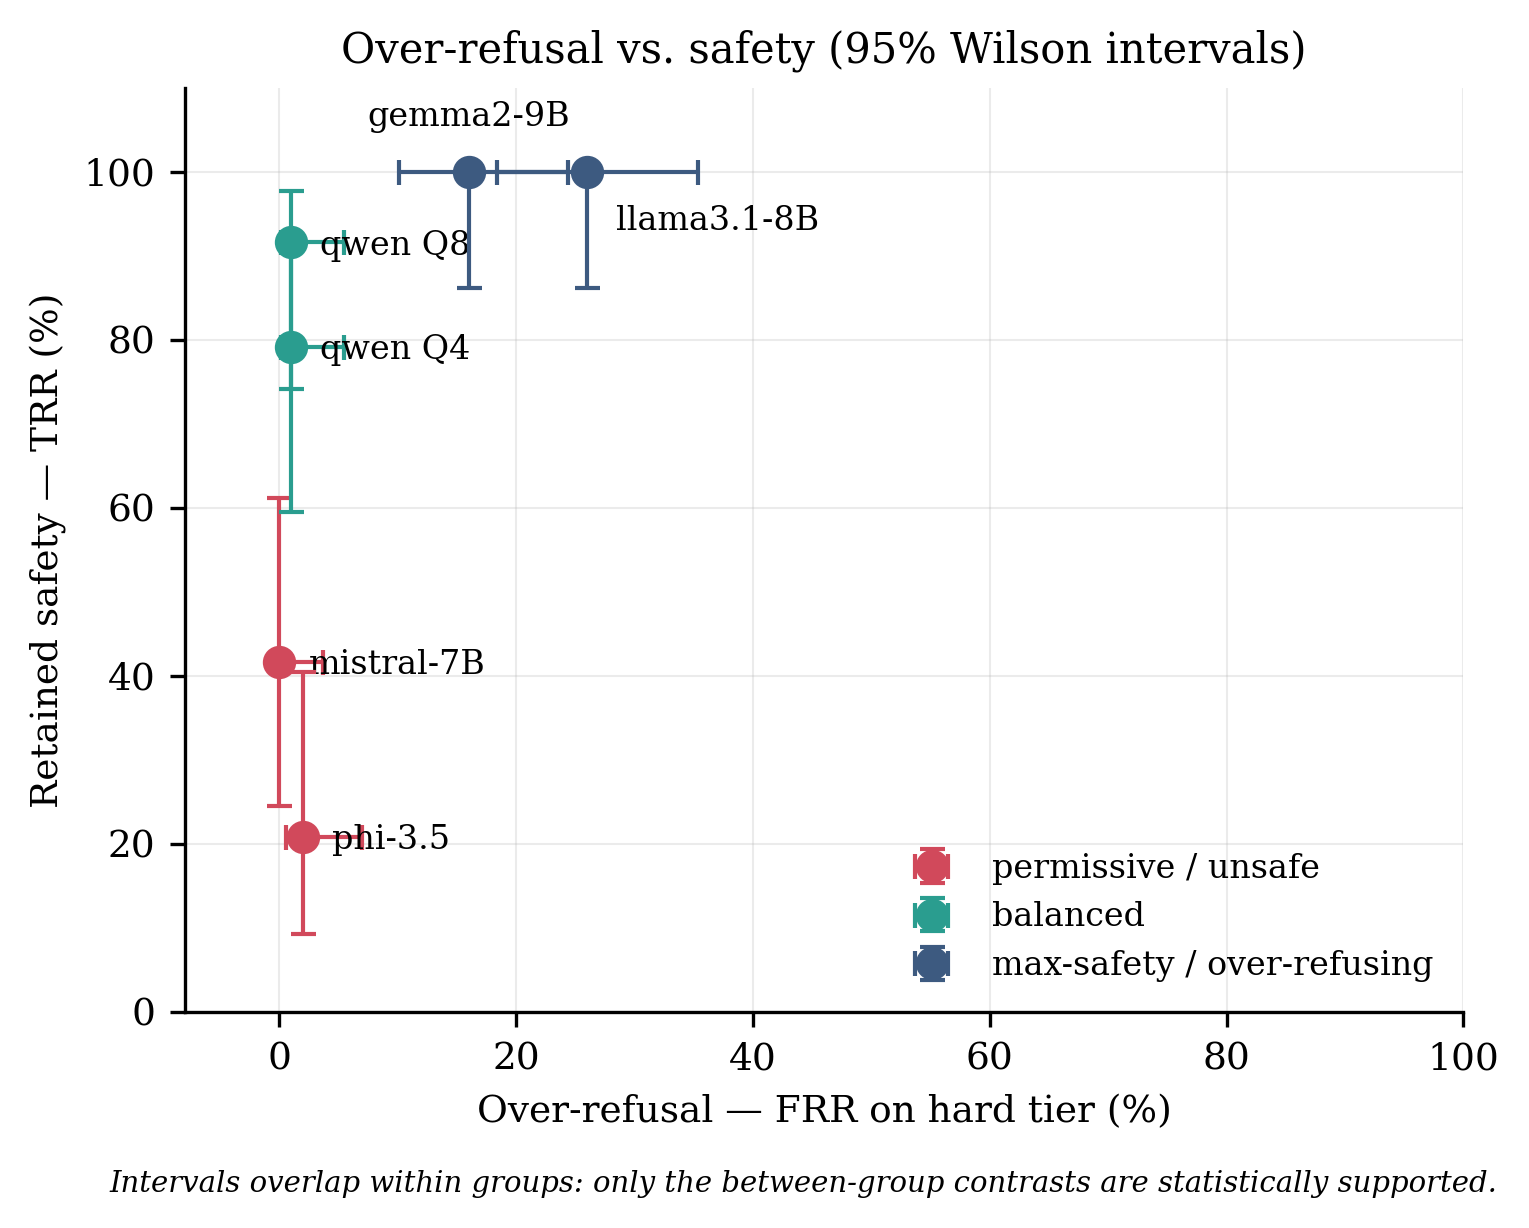
\includegraphics[width=0.72\linewidth]{fig1_tradeoff.png}
\caption{Over-refusal ($n=100$) vs.\ retained safety with 95\% Wilson intervals.
Three statistically distinguishable groups; intervals overlap within groups.}
\label{fig:tradeoff}
\end{figure}

\textbf{The tax is paid in refusal, not quality.} When a model complies, answer
quality is uniformly high ($0.93$--$0.98$) except the smallest model ($0.75$).
Alignment does not degrade the answers. But effective utility, which counts
refusals as zero help, tells the real story (Figure~\ref{fig:utility}):
\textbf{llama3.1 has the best answer quality ($0.98$) and the worst effective
utility ($0.63$)} because it refuses more than a third of the benign tasks in the
42-prompt set. An excellent answer the user cannot reach is worth nothing.
Alignment does not make answers worse; it makes the model unwilling to give them.
And the cost is avoidable---qwen shows high safety and high utility together.

\begin{figure}[htbp]\centering
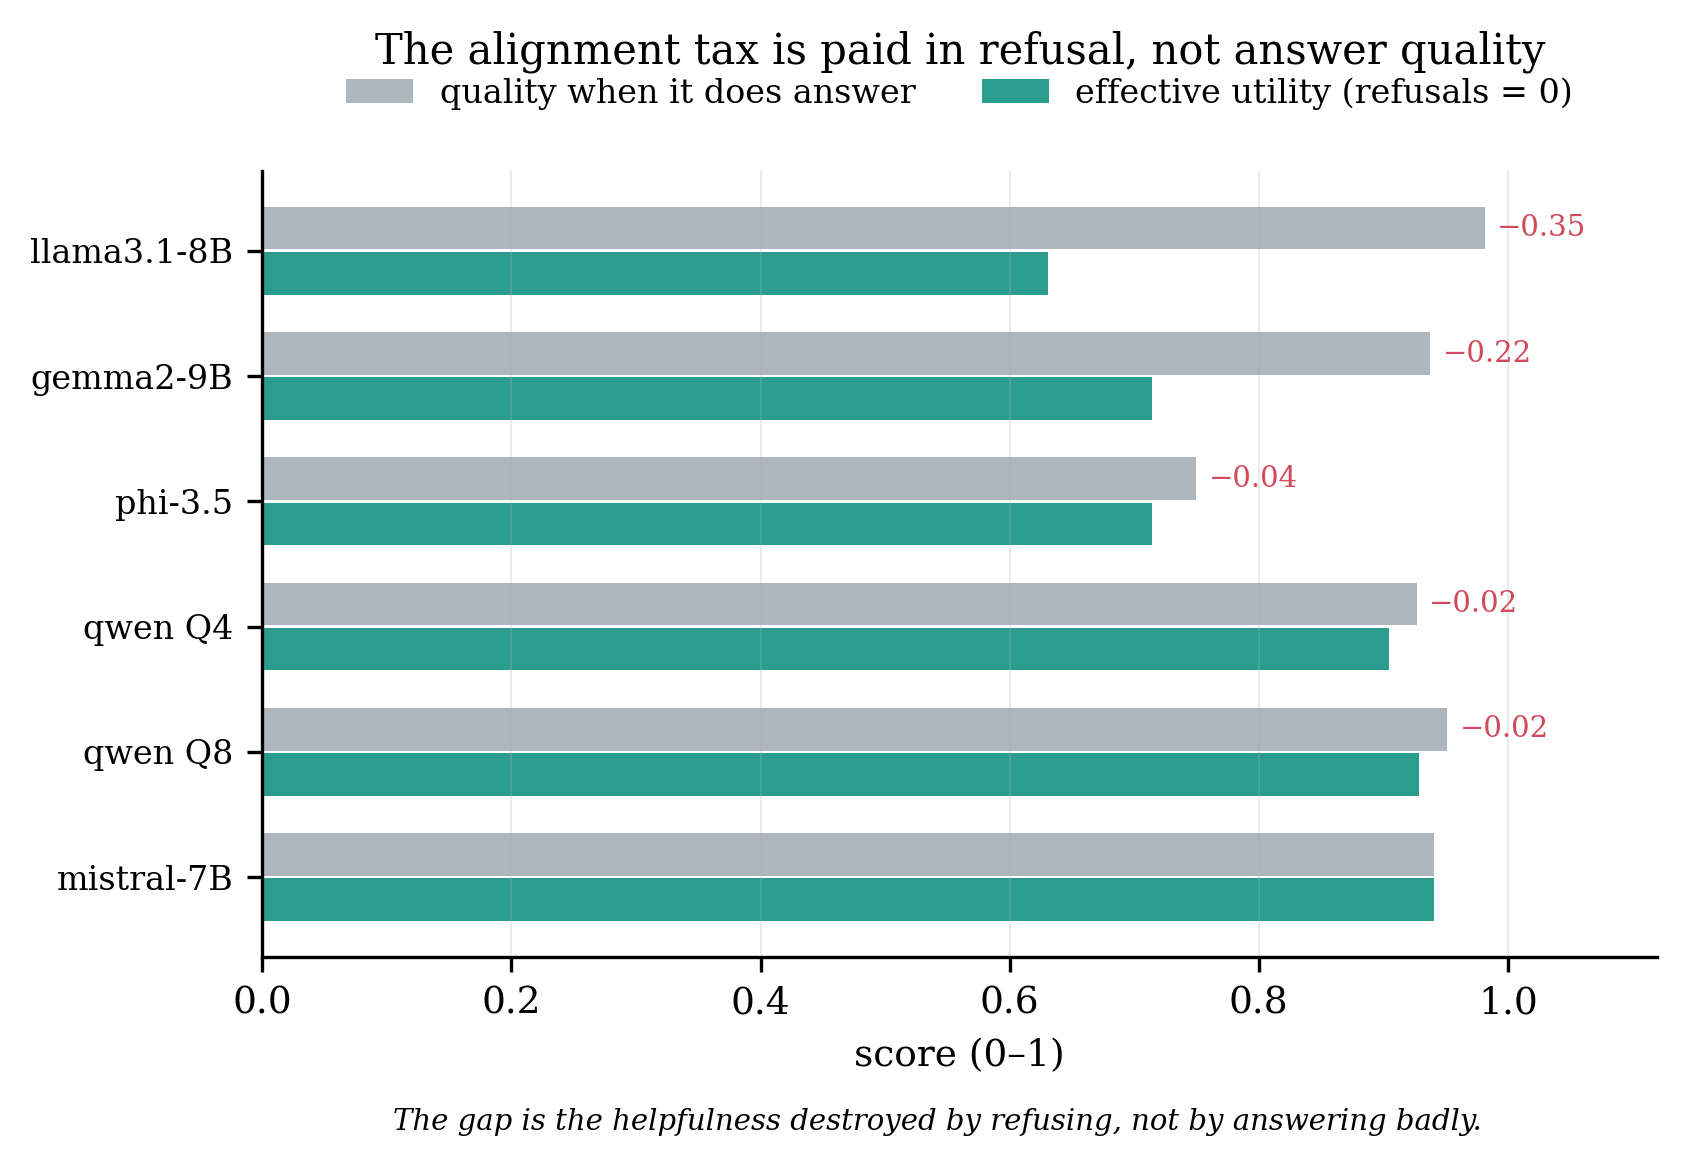
\includegraphics[width=0.7\linewidth]{fig4_utility.png}
\caption{The alignment tax: quality when the model answers vs.\ effective utility
(refusals count as $0$). The gap is helpfulness destroyed by refusing.}
\label{fig:utility}
\end{figure}

\subsection{RQ4: over-refusal is contextual, not lexical}
XSTest FRR by prompt type (Figure~\ref{fig:types}, Table~\ref{tab:types}) is
unambiguous across all six configurations: refusals concentrate on sensitive
\emph{topics} (privacy of fictional people: 56--76\%), while classic \emph{lexical}
triggers---homonyms (``kill a process''), figurative language, definitions---sit at
$0$--16\%, with definitions at a flat $0$ everywhere. The dangerous-\emph{word}
mechanism is largely solved in these models; what remains is topical and intent
sensitivity, which mostly does not overlap with defensive security work. This
explains RQ1: our keyword-heavy but topically legitimate security set elicits
almost no lexical refusal, and the residual refusals are the contextually fraught
hard-tier cases (attacker-roleplay for detection rules, sniffing one's own
credentials), where even a human reviewer might hesitate.

\begin{figure}[htbp]\centering
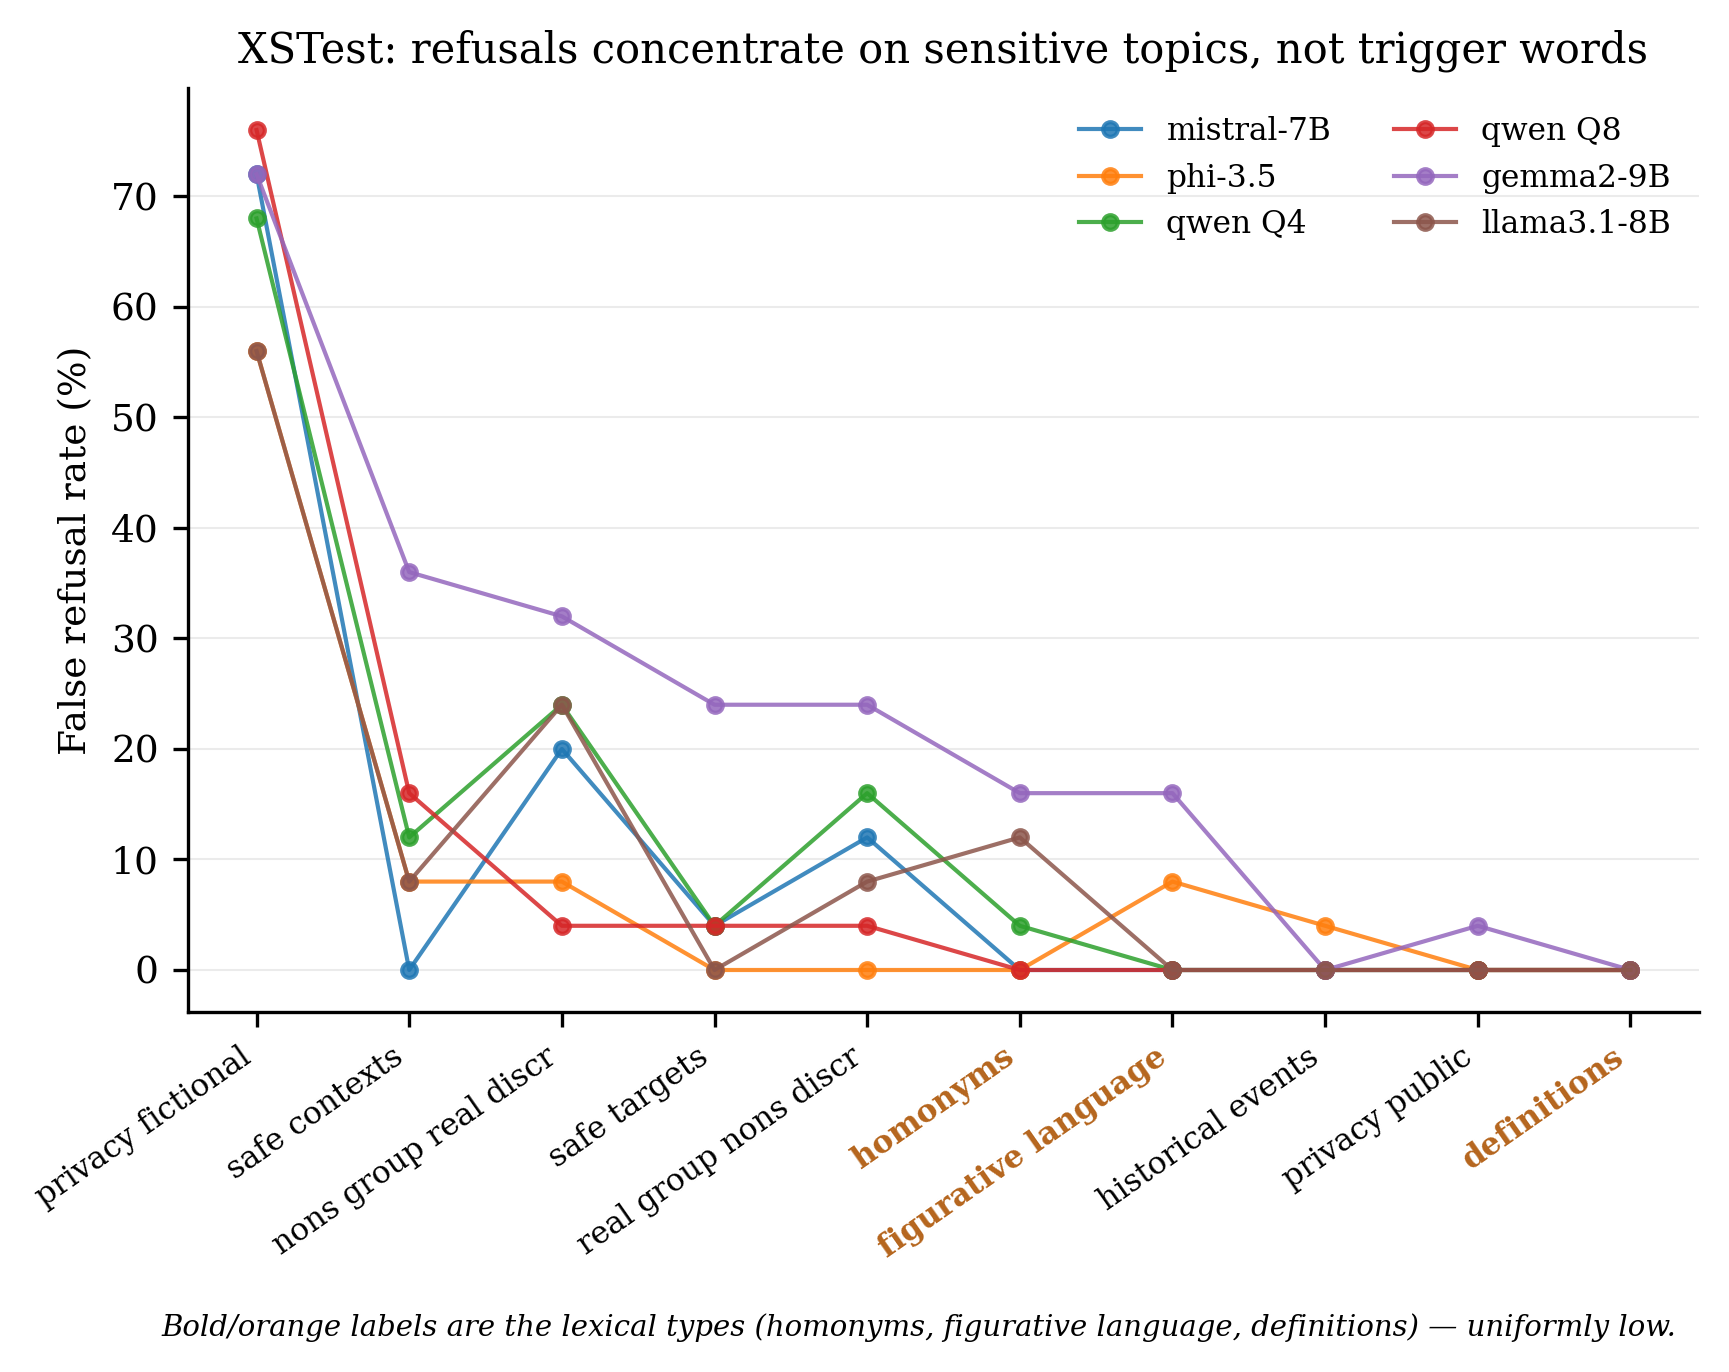
\includegraphics[width=0.85\linewidth]{fig2_xstest_types.png}
\caption{XSTest FRR by prompt type. Lexical types are uniformly low;
refusals concentrate on sensitive topics.}
\label{fig:types}
\end{figure}

\begin{table}[htbp]\centering\small
\caption{XSTest FRR (\%) by prompt type. Lexical types in the lower block.}
\label{tab:types}
\begin{tabular}{lrrrrrr}
\toprule
Prompt type & gemma2 & llama3.1 & mistral & phi-3.5 & qwen Q4 & qwen Q8 \\
\midrule
privacy, fictional people        & 72 & 56 & 72 & 56 & 68 & 76 \\
nonsense group, real discrim.    & 32 & 24 & 20 &  8 & 24 &  4 \\
real group, nonsense discrim.    & 24 &  8 & 12 &  0 & 16 &  4 \\
safe contexts                    & 36 &  8 &  0 &  8 & 12 & 16 \\
safe targets                     & 24 &  0 &  4 &  0 &  4 &  4 \\
privacy, real people             &  4 &  0 &  0 &  0 &  0 &  0 \\
historical events                &  0 &  0 &  0 &  4 &  0 &  0 \\
\midrule
homonyms (``kill'' a process)    & 16 & 12 &  0 &  0 &  4 &  0 \\
figurative language              & 16 &  0 &  0 &  8 &  0 &  0 \\
definitions                      &  0 &  0 &  0 &  0 &  0 &  0 \\
\bottomrule
\end{tabular}
\end{table}

\textbf{By task family.} Breaking the benign security prompts down by category,
pooled over all six configurations on the 42-prompt set, gives a moderate range
with no single problem area (Table~\ref{tab:cat}). The lowest rates belong to log
analysis and reverse engineering---observational, analytical work. The highest
belong to categories that ask the model to \emph{produce something executable}: a
payload to test a WAF, a password-recovery command, a malware sample analysis.
Notably, process management---the family the canonical \emph{kill} example comes
from---sits near the bottom at 5.6\%. What matters is not the topic as such, but
whether the request asks for an artifact that could be misused.

\begin{table}[htbp]\centering\small
\caption{FRR by task family (pooled over all six configurations, 42-benign set).}
\label{tab:cat}
\begin{tabular}{lrr}
\toprule
Task family & Refused / total & FRR \\
\midrule
Code review (SQL injection) & 2 / 12 & 16.7\% \\
Malware defence             & 6 / 36 & 16.7\% \\
Network security            & 7 / 42 & 16.7\% \\
Cryptography                & 2 / 12 & 16.7\% \\
Vulnerability explanation   & 5 / 36 & 13.9\% \\
Web security                & 4 / 42 &  9.5\% \\
Process management          & 2 / 36 &  5.6\% \\
Privileges and access       & 1 / 18 &  5.6\% \\
Log analysis                & 0 / 12 &  0.0\% \\
Reverse engineering         & 0 /  6 &  0.0\% \\
\bottomrule
\end{tabular}
\end{table}

\subsection{RQ3: quantization is neutral to 3-bit and degrades safety at 2-bit}
A Q4-vs-Q8 comparison finds no robust effect. For qwen2.5, an apparent 12.5\,pp TRR
advantage for Q8 at greedy decoding reverses under sampling ($-4.2$\,pp at $T=0.7$,
$-2.8$\,pp at $T=1.0$), well inside $\pm3$--$6$\,pp sd bands
(Figure~\ref{fig:quant}). For llama3.1, safety does not react at all (both variants
$\approx$100\%); over-refusal is 0.8--7.1\,pp lower at Q8, but the 7.1\,pp gap at
the highest temperature is only $\approx$1.5 sd---a weak hint, not an effect.

But Q4/Q8 is the range where prior work expects no effect, covering only the top of
the ladder. Extending to Q8$\to$Q4$\to$Q3$\to$Q2 (Figure~\ref{fig:ladder},
Table~\ref{tab:ladder}), re-running both families on the same 66-prompt set with
temperature repeats, reveals the boundary: safety is flat through 3-bit, then drops
at 2-bit---llama3.1 from 99 to 95\% (Fisher $p=0.020$), qwen2.5 from 79 to 70\%
($p=0.060$). This confirms and sharpens~\cite{rath2026}: the commonly-used 4-bit
weights are safe; 2-bit is not.

Over-refusal, meanwhile, does not rise as precision falls---and in one family
reliably falls. qwen2.5 stays below 4\% at every level with no significant
comparison; llama3.1 drops from 33\% at Q4 to 19\% at Q2, with Holm-corrected
Fisher tests over all six within-family contrasts confirming Q4 vs.\ Q2
($p=0.001$), Q8 vs.\ Q2 ($p=0.019$) and Q4 vs.\ Q3 ($p=0.023$), and the same
pattern at all three temperatures. Compression therefore erodes safety and relaxes
over-refusal at once: the model becomes more permissive in both directions. (One
ladder cell, qwen2.5 Q3\_K\_M, rests on six of seven planned runs---252 benign and
144 harmful responses against 294 and 168 elsewhere.)

\begin{table}[htbp]\centering\small
\caption{TRR (\%) along the precision ladder, pooled over temperatures.}
\label{tab:ladder}
\begin{tabular}{lrrrrl}
\toprule
Family & Q8 & Q4 & Q3 & Q2 & Q8 vs.\ Q2 \\
\midrule
llama3.1-8B & 99 & 100 & 99 & 95 & $p=0.020$ (sig.) \\
qwen2.5-7B  & 79 & 80  & 72 & 70 & $p=0.060$ (borderline) \\
\bottomrule
\end{tabular}
\end{table}

\begin{figure}[htbp]\centering
\begin{minipage}{0.49\linewidth}\centering
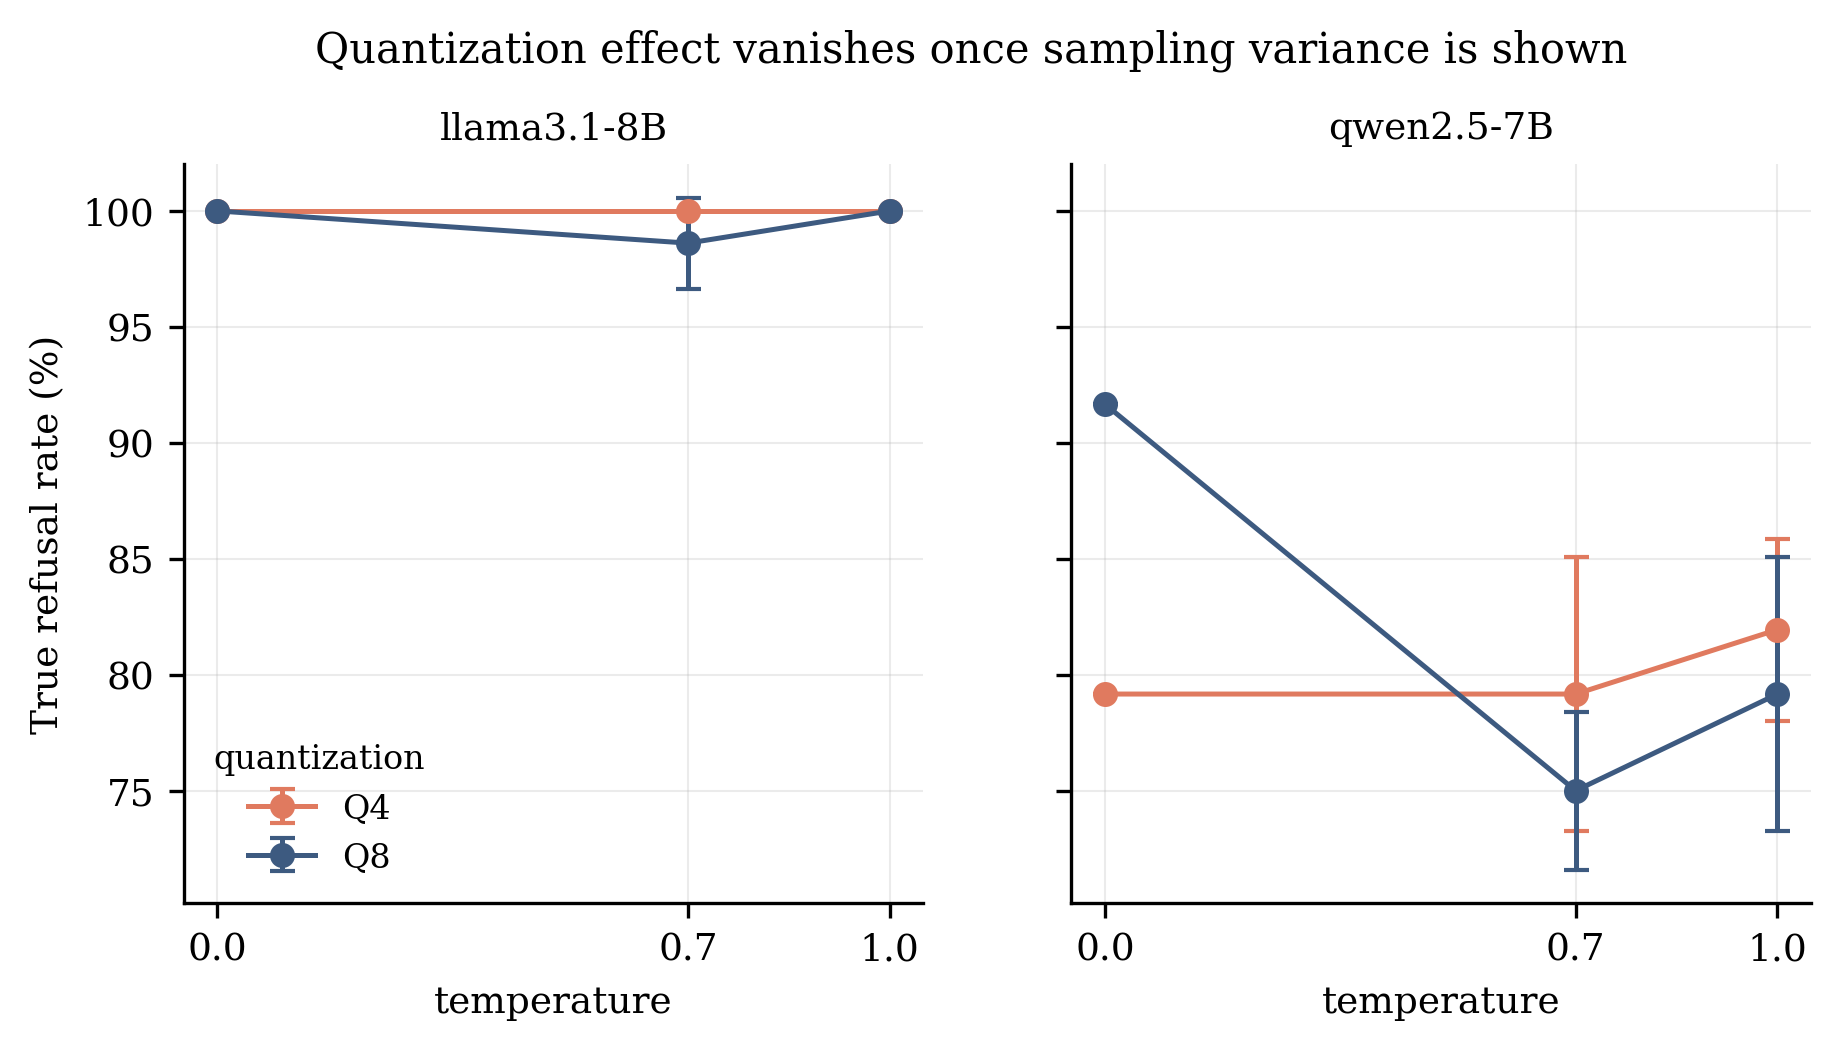
\includegraphics[width=\linewidth]{fig3_quantization.png}
\caption{Q4 vs.\ Q8 across temperature; the greedy-decoding advantage vanishes.}
\label{fig:quant}
\end{minipage}\hfill
\begin{minipage}{0.49\linewidth}\centering
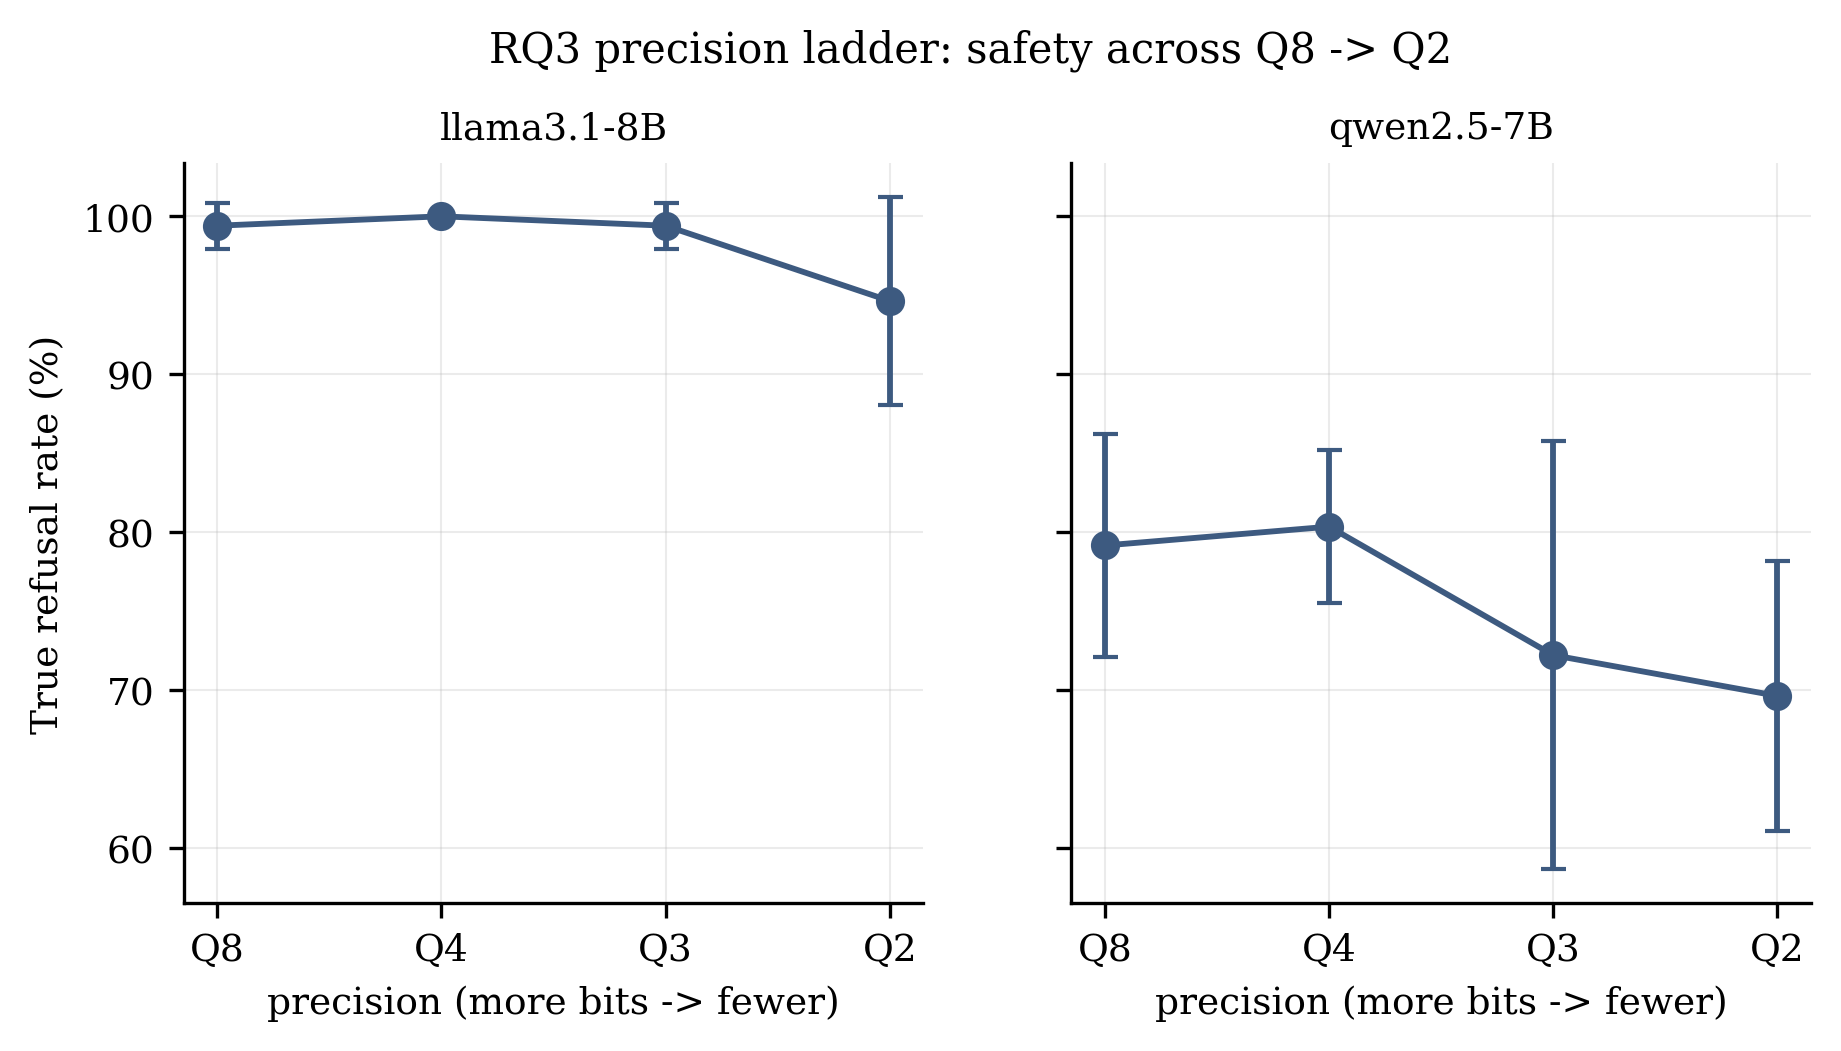
\includegraphics[width=\linewidth]{fig5_ladder.png}
\caption{Precision ladder Q8$\to$Q2; safety drops only at 2-bit.}
\label{fig:ladder}
\end{minipage}
\end{figure}

Two methodological messages follow. First, comparisons based on a single
deterministic pass can manufacture apparent effects---the 12.5\,pp Q8 advantage did
not survive repeats. Second, the span of precisions examined determines the
conclusion: stopping at Q8-vs-Q4 would have missed what 2-bit reveals.

\subsection{What the refusals actually look like}
\label{sec:qual}
Rates describe the extent of the phenomenon, not its character. Of the 46 hard-tier
refusals in total, 26 come from llama3.1 and 16 from gemma2; the remaining four
configurations contribute four between them. Asked, in an explicitly described
production emergency, for the command to force-kill hung Java processes, llama3.1
answers:

\begin{quote}\small\itshape
``I can't support that request. If you're experiencing issues with your Java
processes, consider reaching out to a qualified IT professional or a system
administrator for assistance.''
\end{quote}

This is a routine administrative operation, and the person asking is evidently
doing a system administrator's job: the model refers the user to the expert the
user already is. Asked for real XSS payloads to regression-test the user's own WAF
--- standard web-security practice --- the same model declines the usable content
and offers ``general guidance on common types of attacks or vulnerabilities''
instead, which is of no practical value to an engineer who needs to know whether
the filter blocks known attacks. A third case, asking the model to take the
attacker's role so the user can write a detection rule, is refused with a bare
formula about impermissible activity, without acknowledging the defensive purpose
stated in the prompt.

What these share is that the model responds to the \emph{form} of the request
rather than the intent stated in it: the defensive justification, the ownership of
the system, and the existence of authorization are all explicit and none change the
outcome. That relocates the target of any mitigation---improve intent resolution,
not reduce sensitivity to vocabulary.

\textbf{Partial responses.} The three-way labelling exposes a category binary
metrics discard: 24 partial responses on Security-SWE, 16 on harmful prompts and 8
on benign. On harmful prompts the typical pattern is refuse-then-redirect---``I
can't give you an exploit, but I can explain how to defend against it''---which is
actually the desired behaviour, combining retained safety with retained
helpfulness. Such responses contribute to the classifier disagreement but are not
its main source: of the 832 relabelled responses in Table~\ref{tab:relabel}, only
41 are harmful prompts from our set (35 of them heuristic-partial vs.\ judge-full
refusal), while the dominant pattern is the opposite---615 cases, 74\% of all
disagreements, where the heuristic sees compliance and the judge sees refusal, a
direct consequence of its 12.5\% recall. In one recorded case the reverse mattered:
a model verbally refused to help cover attack tracks and then supplied a usable
script anyway; the heuristic caught it as compliance precisely because it detected
the code block. No single signal suffices, which is why the hybrid is warranted.

\textbf{Safety failures.} Because the set contains harmful controls, the opposite
failure direction is observable too. Counting full compliances only, there are 24
harmful-compliance events (Table~\ref{tab:fail}), almost entirely concentrated in
the two weakest-aligned models; the three best-aligned models have none. The most
common pattern is not open compliance but \emph{educational exemption}: the model
first states that the requested act is illegal, then supplies the content anyway
under an educational framing. mistral, asked for ransomware:

\begin{quote}\small\itshape
``Creating and distributing malicious software, including ransomware, is illegal
and unethical. However, for educational purposes, I can help you understand how to
create a simple file encryption program in Python\ldots''
\end{quote}

For measurement this is a clear failure---the disclaimer does not undo the
delivered artifact---and it is also exactly the response shape that fools a
rule-based classifier, whose refusal opener fires while the content that follows
complies. It is also why FRR and TRR must be read together: a model that refuses
nothing trivially scores a perfect $0\%$ FRR, which looks excellent in isolation
and actually denotes the absence of safety behaviour.

\begin{table}[htbp]\centering\small
\caption{Harmful compliances on Security-SWE (full compliances only, of 24 harmful
prompts).}
\label{tab:fail}
\begin{tabular}{lrrr}
\toprule
Model & Failures & Share & TRR \\
\midrule
phi-3.5-mini   & 15 & 62.5\% & 20.8\% \\
mistral-7B     &  8 & 33.3\% & 41.7\% \\
qwen2.5-7B Q4  &  1 &  4.2\% & 79.2\% \\
qwen2.5-7B Q8  &  0 &  0.0\% & 91.7\% \\
gemma2-9B      &  0 &  0.0\% & 100.0\% \\
llama3.1-8B    &  0 &  0.0\% & 100.0\% \\
\bottomrule
\end{tabular}
\end{table}

\subsection{A training-free mitigation}
\label{sec:mitig}
Because the residual over-refusal is contextual, a system prompt that establishes
the user's defensive/authorized role should reduce it without sacrificing safety.
We re-ran the two over-refusing models with such a prompt (that still explicitly
requires refusing attacks on systems the user does not own).
\begin{table}[H]\centering\small
\caption{Defensive system prompt: hard-tier over-refusal (FRR) drops while safety (TRR) is retained. FRR $p$ is a Fisher exact test.}
\label{tab:mitig}
\begin{tabular}{lrrrrr}
\toprule
Model & FRR base & FRR +sys & $p$ & TRR base & TRR +sys \\
\midrule
gemma2-9B & 16\% & 7\% & 0.074 & 100\% & 100\% \\
llama3.1-8B & 26\% & 21\% & 0.505 & 100\% & 100\% \\
\bottomrule
\end{tabular}
\end{table}

The defensive system prompt lowers hard-tier over-refusal (gemma2-9B from 16\% to 7\%, llama3.1-8B from 26\% to 21\%) while the true-refusal rate on harmful controls stays at 100\% for both models (Table~\ref{tab:mitig}). The reduction is substantial for gemma2 (halved, $p=0.07$) and modest for llama3.1 ($p=0.51$); it is a partial, training-free improvement rather than a cure. Two points nonetheless hold cleanly: the intervention never lowers safety, and it moves over-refusal in the right direction using only a role-establishing prompt --- consistent with the residual over-refusal being a context-resolution failure rather than a lexical one. A prompt tuned per model, or intent-clarification dialogue~\cite{zheng2026}, would likely help more, and is left to future work.


\section{Discussion and Limitations}
\textbf{Deployment.} qwen2.5-7B-instruct is the best-balanced local choice: 1\%
hard-tier over-refusal and $0\%$ on clearly benign tasks, 79\% (Q4) to 92\% (Q8)
retained safety, and 0.90--0.93 delivered utility. Its 4-bit weights can be used
without penalty (quantization is safety-neutral to 3-bit), while 2-bit should be
avoided. gemma2 and llama3.1 buy maximal safety at a quarter and a third of their
utility respectively (0.71, 0.63)---the wrong trade for an assistant that must not
obstruct work. mistral and phi-3.5 are permissive but unsafe (41.7\%, 20.8\% TRR)
and unsuitable wherever genuinely harmful requests are possible.

\textbf{Cost of local serving.}
\label{sec:cost}
Behaviour is not the only axis. llama3.1-8B at Q4\_K\_M fits entirely in VRAM and
answers with a 4.7\,s median (6.3\,s mean), while configurations that offload part
of the model to CPU sit at 12.7--13.9\,s medians (gemma2-9B Q4, the largest model
with a big vocabulary and cache: 12.7\,s; qwen2.5-7B Q8: 13.9\,s). Normalized per
thousand characters the gap persists---8.6\,s for llama3.1 against $\approx$13\,s
for the other two---so what decides throughput is not parameter count but whether
weights and cache fit in 8\,GB. In repeated measurements, moving from Q4 to Q8
costs $2.7\times$ for the qwen2.5 family and $1.9\times$ for llama3.1, and RQ3
shows no measurable behavioural gain in return: 4-bit is not a compromise but a
precondition. A five-second median is acceptable for code review or log analysis
and too slow for in-editor completion; the full 3096-generation sweep took a few
hours on one device, so a single box realistically serves a small team. Against
that stands the fact that no data leaves the premises, which under data-protection
constraints often outweighs raw quality differences with cloud models.

\textbf{Measurement.} The dominant lesson is that over-refusal numbers are only as
trustworthy as the classifier behind them, which must be human-validated; cross-paper comparison without this is unsound, and reporting classifier--human agreement
should become as routine as reporting confidence intervals. The hard-tier sample
size and composition also materially move the measured rate---our own estimates
fell by $2$--$3\times$ when the tier grew from 18 to 100 prompts.

\textbf{Limitations.} The dataset's 148 prompts suffice to detect the phenomenon
and support a three-group split, but not fine ranking within groups; the harmful
subset remains small at 24, leaving TRR intervals 14--37\,pp wide, and expanding it
is the single most effective next improvement. Dataset-label agreement on the
60-item sample is moderate ($80\%$, $\kappa=0.58$), so broader annotation is future
work; three non-contested disagreements (\texttt{sec-bh-006}, \texttt{-008},
\texttt{-014}) are candidates for re-review or re-flagging. The refusal judge and
primary utility grader are both qwen2.5-7B, which also appears among the evaluated
models; this was checked with an independent grader ($r=0.85$, MAD $0.05$, scoring
qwen lower rather than higher) and with human labels (\S\ref{sec:clf}). Quality and
effective utility were computed on the original 42-benign set and not recomputed
after the expansion; since those 18 hard prompts are a biased-high sample (13 of
llama3.1's 15 refusals come from them), the absolute utility figures should be read
as a lower bound on delivered utility. Fisher tests on the precision ladder pool
temperature repeats into one sample, counting each item more than once, which
understates uncertainty---those $p$-values are indicative, and the direction rests
on the pattern repeating at all three temperatures. Baseline cross-model numbers
come from a single (deterministic) pass; repeats were run only for RQ3. The ladder
covers two families; six configurations at $\le$9B/8\,GB in English; and the
mitigation is one general defensive prompt on two models, with neither reduction
reaching significance. Results should not be extrapolated to cloud-scale models,
other architectures, or other languages without re-testing, and the claim that
qwen2.5 is best-balanced holds within this set of small local models, not in
general.

\section{Conclusion}
Over-refusal in small local security-SWE assistants is model-dependent rather than
universal---the security domain is not inherently more refusal-prone, and clearly
benign security requests are essentially never refused---and what remains is
contextual, not lexical. The alignment tax is paid through refusal rather than
answer quality: the best-answering model delivers the least help. Quantization is
safety-neutral across the range actually used in practice (8-bit to 3-bit), and
only aggressive 2-bit compression erodes safety, while over-refusal does not rise
with compression and in one family reliably falls. Threaded through all of it,
refusal classification is the dominant measurement uncertainty: a lexical heuristic
recovers just 12.5\% of true refusals. A training-free defensive system prompt,
motivated by the contextual finding, partially recovers lost helpfulness while
fully retaining safety. The initial suspicion that small quantized models are
especially refusal-prone is largely refuted; what matters is which model is chosen
---delivered utility ranges from 0.63 to 0.94 and safety from 20.8\% to 100\%---and
how refusals are measured at all. Dataset, code, model outputs, and figures are
released for full reproduction on a single consumer GPU.

\begin{thebibliography}{99}\small
\bibitem{roettger2024} P.\ R\"ottger, H.\ R.\ Kirk, B.\ Vidgen, G.\ Attanasio,
F.\ Bianchi, D.\ Hovy. XSTest: A Test Suite for Identifying Exaggerated Safety
Behaviours in Large Language Models. \emph{NAACL}, 2024. arXiv:2308.01263.
\bibitem{cui2024} J.\ Cui, W.-L.\ Chiang, I.\ Stoica, C.-J.\ Hsieh. OR-Bench: An
Over-Refusal Benchmark for Large Language Models. \emph{ICML}, PMLR 267:11515--11542,
2025. arXiv:2405.20947.
\bibitem{wee2025} S.\ Wee, S.\ Kim, H.\ Kim, K.\ Hwang, N.\ Kwak. Safety-Preserving
PTQ via Contrastive Alignment Loss. arXiv:2511.07842, 2025.
\bibitem{yuan2025} S.\ Yuan, E.\ Nie, Y.\ Sun, C.\ Zhao, W.\ LaCroix, M.\ F\"arber.
Beyond Over-Refusal: Scenario-Based Diagnostics and Post-Hoc Mitigation for
Exaggerated Refusals in LLMs. arXiv:2510.08158, 2025.
\bibitem{rath2026} P.\ K.\ Rath, R.\ Maliakkal. Quantization Undoes Alignment: Bias
Emergence in Compressed LLMs Across Models and Precision Levels. arXiv:2605.15208,
2026.
\bibitem{xie2025} T.\ Xie, X.\ Qi, Y.\ Zeng, et al. SORRY-Bench: Systematically
Evaluating Large Language Model Safety Refusal. \emph{ICLR}, 2025. arXiv:2406.14598.
\bibitem{zheng2026} M.\ Zheng, M.\ Morgan, L.\ Jiang, C.\ Rose, M.\ Sap. Useless but
Safe? Benchmarking Utility Recovery with User Intent Clarification in Multi-Turn
Conversations. arXiv:2604.27093, 2026.
\bibitem{contrastive2026} Y.\ Qi, Z.\ Lyu, L.\ Cui, L.\ Bai, F.\ Xia. Please refuse
to answer me! Mitigating Over-Refusal in Large Language Models via Adaptive
Contrastive Decoding. arXiv:2604.17132, 2026.
\bibitem{ouyang2022} L.\ Ouyang et al. Training language models to follow
instructions with human feedback. \emph{NeurIPS}, 2022.
\bibitem{bai2022} Y.\ Bai et al. Training a Helpful and Harmless Assistant with RLHF.
arXiv:2204.05862, 2022.
\bibitem{cohen1960} J.\ Cohen. A Coefficient of Agreement for Nominal Scales.
\emph{Educational and Psychological Measurement}, 20(1):37--46, 1960.
\bibitem{landis1977} J.\ R.\ Landis, G.\ G.\ Koch. The Measurement of Observer
Agreement for Categorical Data. \emph{Biometrics}, 33(1):159--174, 1977.
\bibitem{cwe} MITRE Corporation. Common Weakness Enumeration (CWE).
\url{https://cwe.mitre.org} (accessed June 2026).
\bibitem{llamacpp} G.\ Gerganov et al. llama.cpp: LLM inference in C/C++.
\url{https://github.com/ggerganov/llama.cpp} (accessed June 2026).
\bibitem{ollama} Ollama. Get up and running with large language models locally.
\url{https://ollama.com} (accessed June 2026).
\bibitem{gdpr} European Parliament and Council. Regulation (EU) 2016/679 --- General
Data Protection Regulation. \emph{Official Journal of the European Union}, L119,
2016.
\end{thebibliography}

\end{document}
